% Options for packages loaded elsewhere
\PassOptionsToPackage{unicode}{hyperref}
\PassOptionsToPackage{hyphens}{url}
%
\documentclass[
]{article}
\usepackage{amsmath,amssymb}
\usepackage{lmodern}
\usepackage{ifxetex,ifluatex}
\ifnum 0\ifxetex 1\fi\ifluatex 1\fi=0 % if pdftex
  \usepackage[T1]{fontenc}
  \usepackage[utf8]{inputenc}
  \usepackage{textcomp} % provide euro and other symbols
\else % if luatex or xetex
  \usepackage{unicode-math}
  \defaultfontfeatures{Scale=MatchLowercase}
  \defaultfontfeatures[\rmfamily]{Ligatures=TeX,Scale=1}
\fi
% Use upquote if available, for straight quotes in verbatim environments
\IfFileExists{upquote.sty}{\usepackage{upquote}}{}
\IfFileExists{microtype.sty}{% use microtype if available
  \usepackage[]{microtype}
  \UseMicrotypeSet[protrusion]{basicmath} % disable protrusion for tt fonts
}{}
\makeatletter
\@ifundefined{KOMAClassName}{% if non-KOMA class
  \IfFileExists{parskip.sty}{%
    \usepackage{parskip}
  }{% else
    \setlength{\parindent}{0pt}
    \setlength{\parskip}{6pt plus 2pt minus 1pt}}
}{% if KOMA class
  \KOMAoptions{parskip=half}}
\makeatother
\usepackage{xcolor}
\IfFileExists{xurl.sty}{\usepackage{xurl}}{} % add URL line breaks if available
\IfFileExists{bookmark.sty}{\usepackage{bookmark}}{\usepackage{hyperref}}
\hypersetup{
  hidelinks,
  pdfcreator={LaTeX via pandoc}}
\urlstyle{same} % disable monospaced font for URLs
\usepackage[margin=1in]{geometry}
\usepackage{graphicx}
\makeatletter
\def\maxwidth{\ifdim\Gin@nat@width>\linewidth\linewidth\else\Gin@nat@width\fi}
\def\maxheight{\ifdim\Gin@nat@height>\textheight\textheight\else\Gin@nat@height\fi}
\makeatother
% Scale images if necessary, so that they will not overflow the page
% margins by default, and it is still possible to overwrite the defaults
% using explicit options in \includegraphics[width, height, ...]{}
\setkeys{Gin}{width=\maxwidth,height=\maxheight,keepaspectratio}
% Set default figure placement to htbp
\makeatletter
\def\fps@figure{htbp}
\makeatother
\setlength{\emergencystretch}{3em} % prevent overfull lines
\providecommand{\tightlist}{%
  \setlength{\itemsep}{0pt}\setlength{\parskip}{0pt}}
\setcounter{secnumdepth}{-\maxdimen} % remove section numbering
\ifluatex
  \usepackage{selnolig}  % disable illegal ligatures
\fi

\author{true \and true \and true \and true \and true \and true \and true \and true \and true}
\date{}

\begin{document}

\hypertarget{abstract}{%
\section{Abstract}\label{abstract}}

DNA alteration signatures are recurring patterns that are the imprints
of mutagenic processes accumulated during the evolution of cancer cell.
Despite the importance of copy number alteration (CNA) in cancer
progression,comprehensive understanding about the mutational processes
and signatures of CNA is still lacking. Here we developed a method to
categorize CNA based on various fragment properties, which reflect the
consequences of mutagenic processes and can be extracted from different
types of data, including whole genome sequencing (WGS), whole exome
sequencing (WES) and SNP array. The signature of CNA has been extracted
from 2778 pan-cancer analysis of whole genomes (PCAWG) WGS samples, and
further validated using 10851 the cancer genome atlas (TCGA) SNP array
dataset. Novel copy number signatures associated with haploid chromosome
have been identified. The activities of some copy number signatures
consistently predict cancer patients' prognosis. This study provides a
repertoire for understanding the signatures and mutational processes of
CNA.

\hypertarget{methodology}{%
\section{Methodology}\label{methodology}}

\begin{figure}

{\centering \includegraphics[width=0.8\linewidth]{Figures/copy number classification} 

}

\caption{CNA classification strategy for signature analysis.}\label{fig:figure1}
\end{figure}

For each CNA segment, the following features have been considered: 1,
segment context, including segment shape and copy number change number;
2, Absolute copy number; 3, LOH status; 4, segment size. In total 176
types of CNA segments have been defined accordingly.

\begin{figure}

{\centering 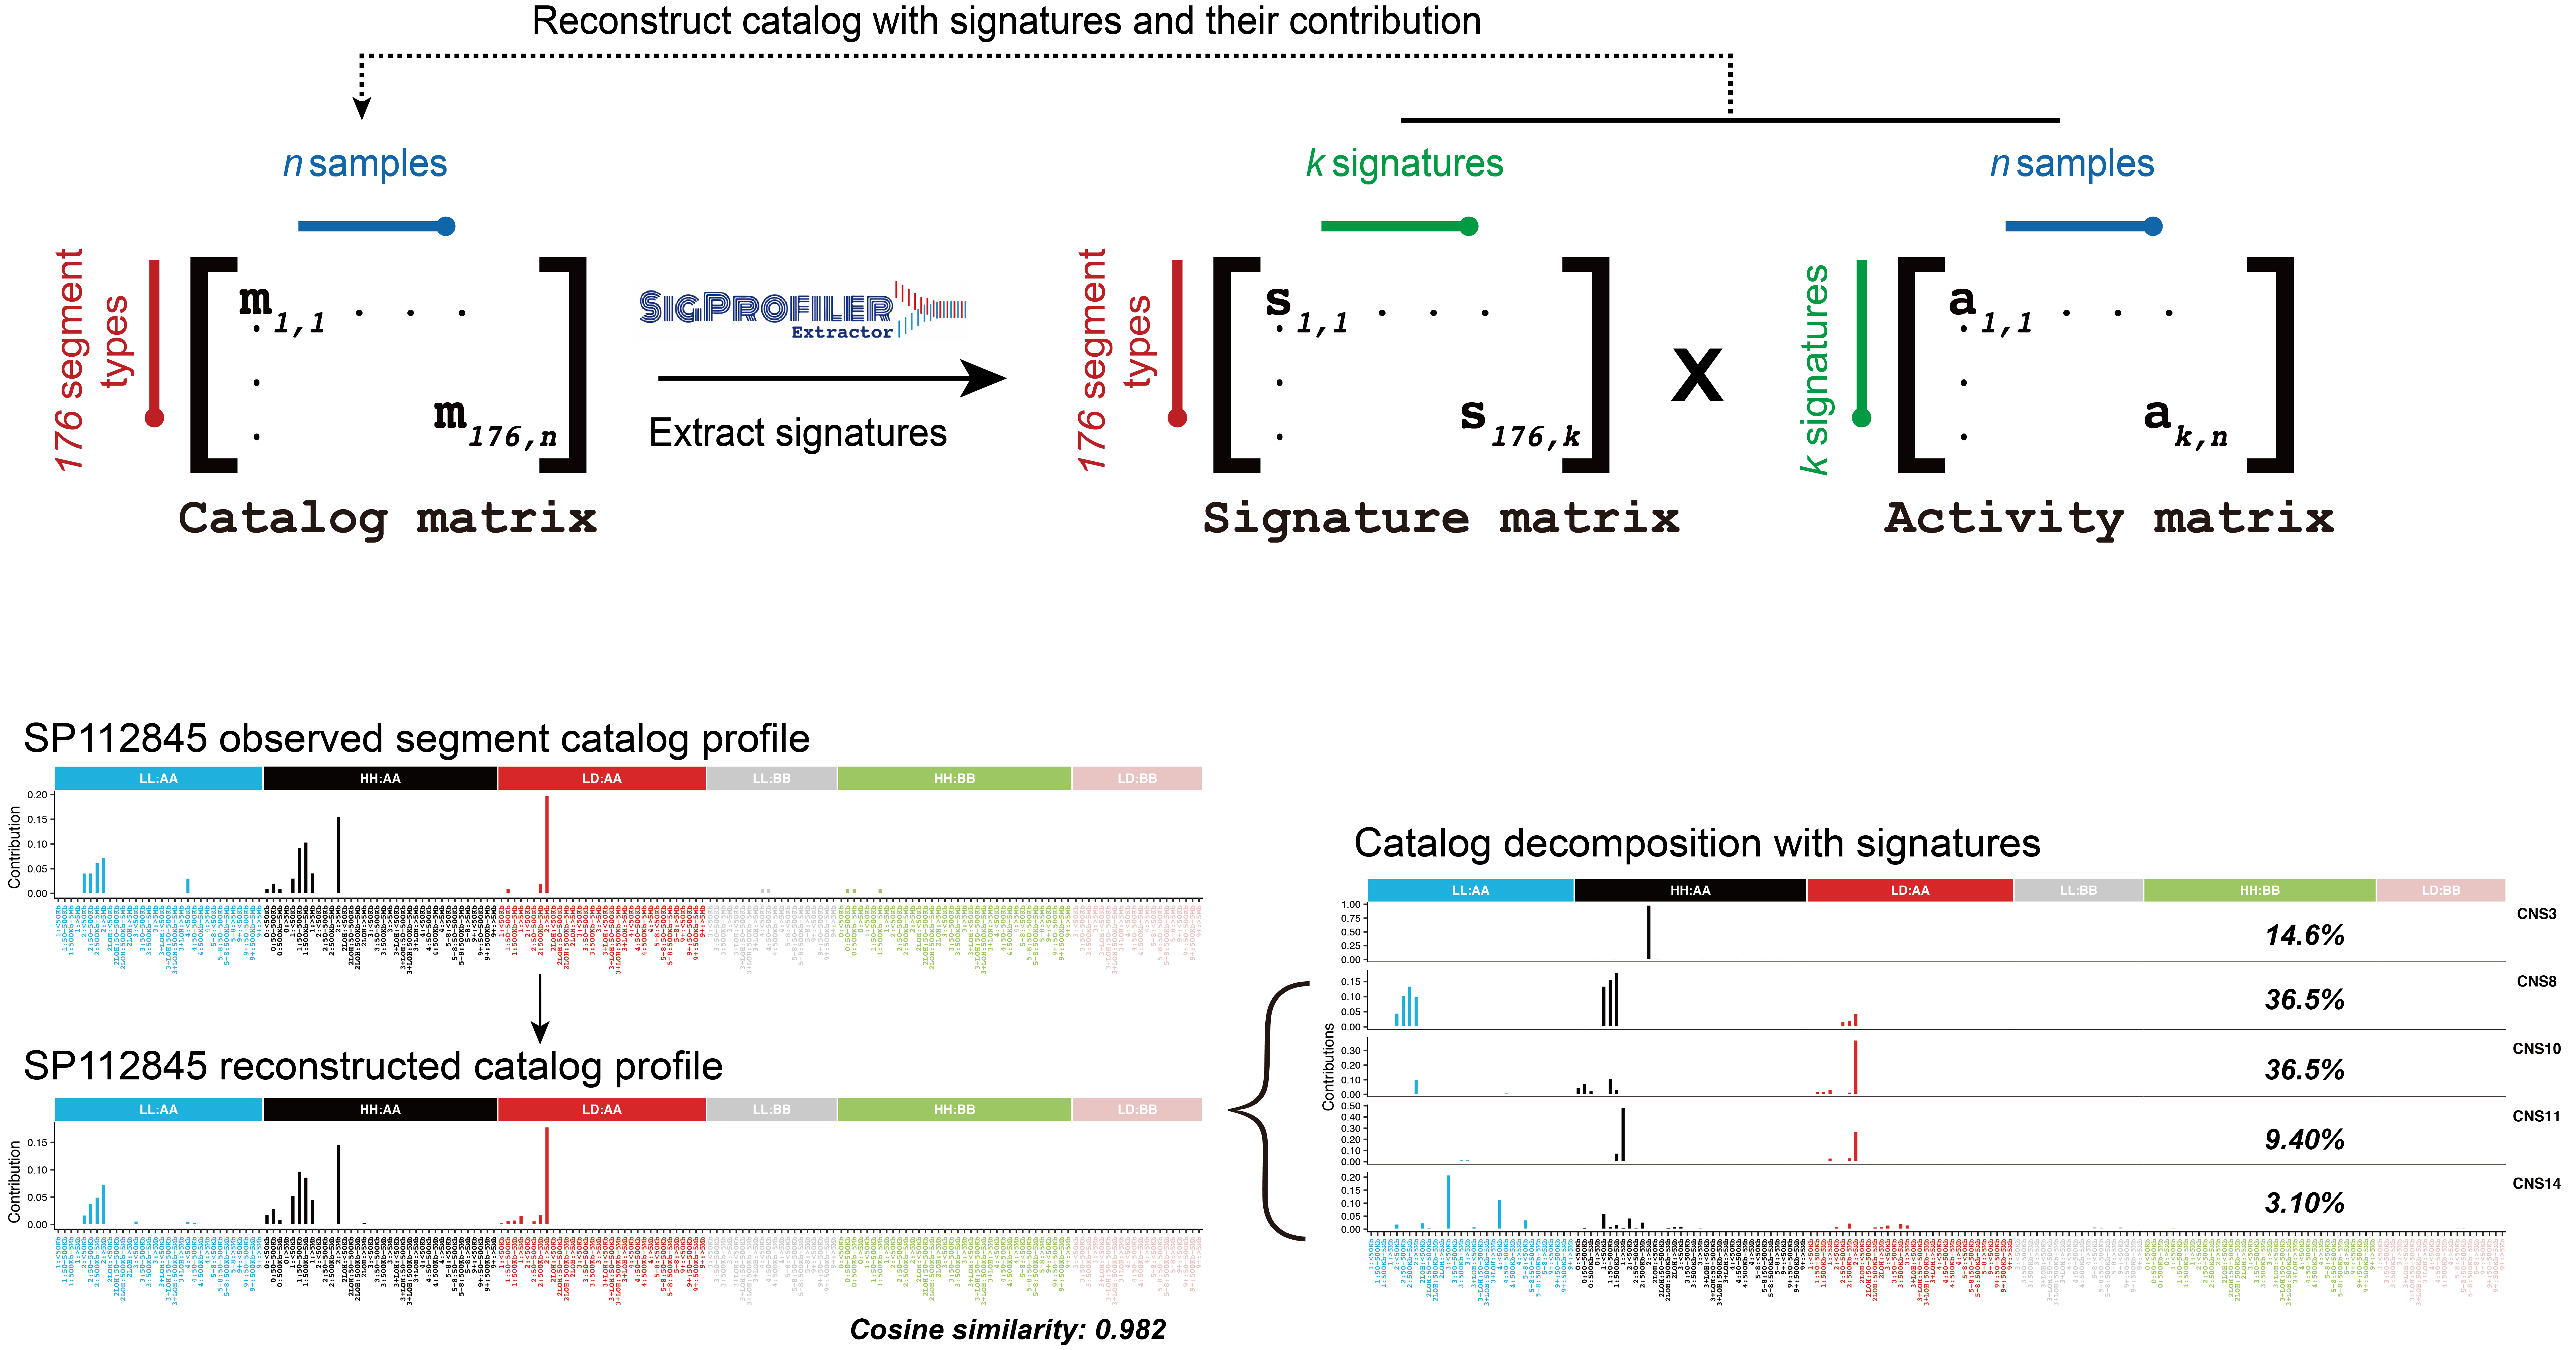
\includegraphics[width=0.8\linewidth]{Figures/extraction} 

}

\caption{De novo CNA signature extraction with sigprofiler.}\label{fig:figure2}
\end{figure}

We selected the signature extraction solution as the maximum signature
number which meets the following criteria: 1. No over fit. 2. Stability
should be at least local maximal. 3. Mean cosine distance should be as
small as possible. Based on the rules, we selected 14 signatures for
PCAWG copy number data.

\hypertarget{results}{%
\section{Results}\label{results}}

\textbackslash begin\{figure\}

\{\centering 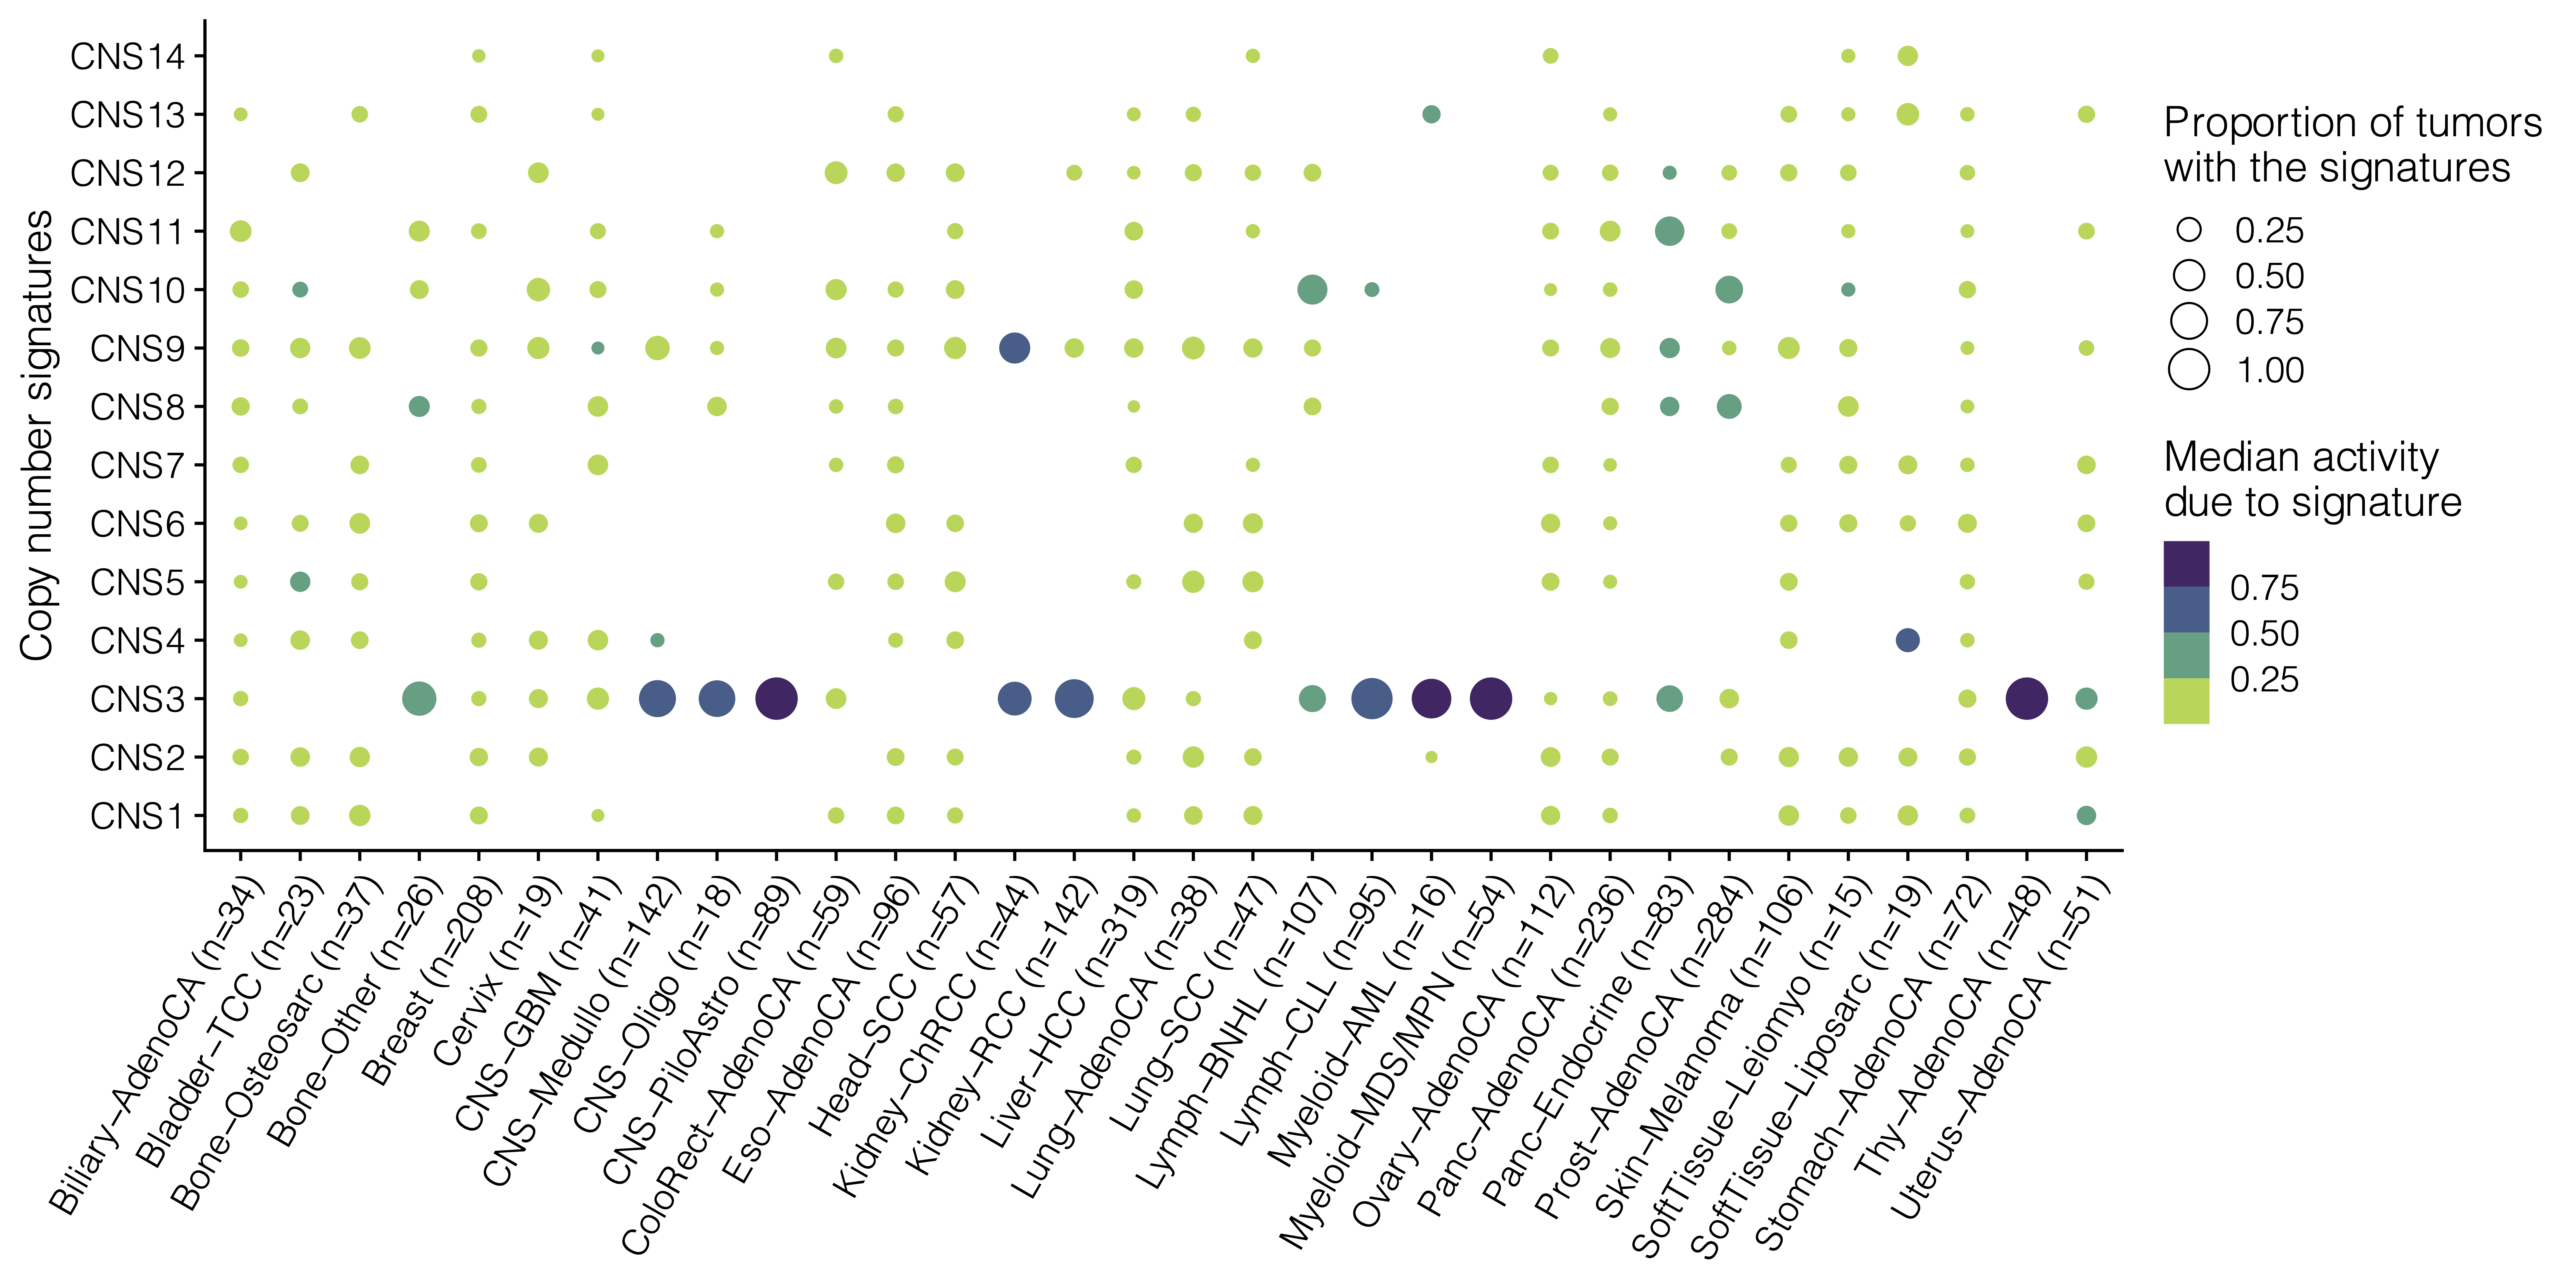
\includegraphics[width=0.7\linewidth]{Figures/CNS_PCAWG_landscape_proportion_0.05}

\}

\textbackslash caption\{Proportion of tumors with the signature and the
median activity of the signature are shown for 32 PCAWG cancer types.
For each individual tumor, only signatures that contribute to ≥5\% of
the total are counted.\}\label{fig:figure3} \textbackslash end\{figure\}

\begin{figure}

{\centering \includegraphics[width=1\linewidth]{Figures/CNS-Profile} 

}

\caption{Representative CNA profile, prominent features and potential mechanisms for each identified CNA signatures extracted in PCAWG dataset.}\label{fig:figure4}
\end{figure}

An important purpose of CNA signature analysis is to identify the
underlying mutational processes for CNA, and classify CNA based on
mutational processes. Potential mutational processes for CNA include
intrinsic inducers and extrinsic inducers. Intrinsic CNA inducers
include: double-strand break repair defect (HRD etc.); cell cycle
defect; DNA replication defects; telomere loss, etc.

\begin{figure}

{\centering 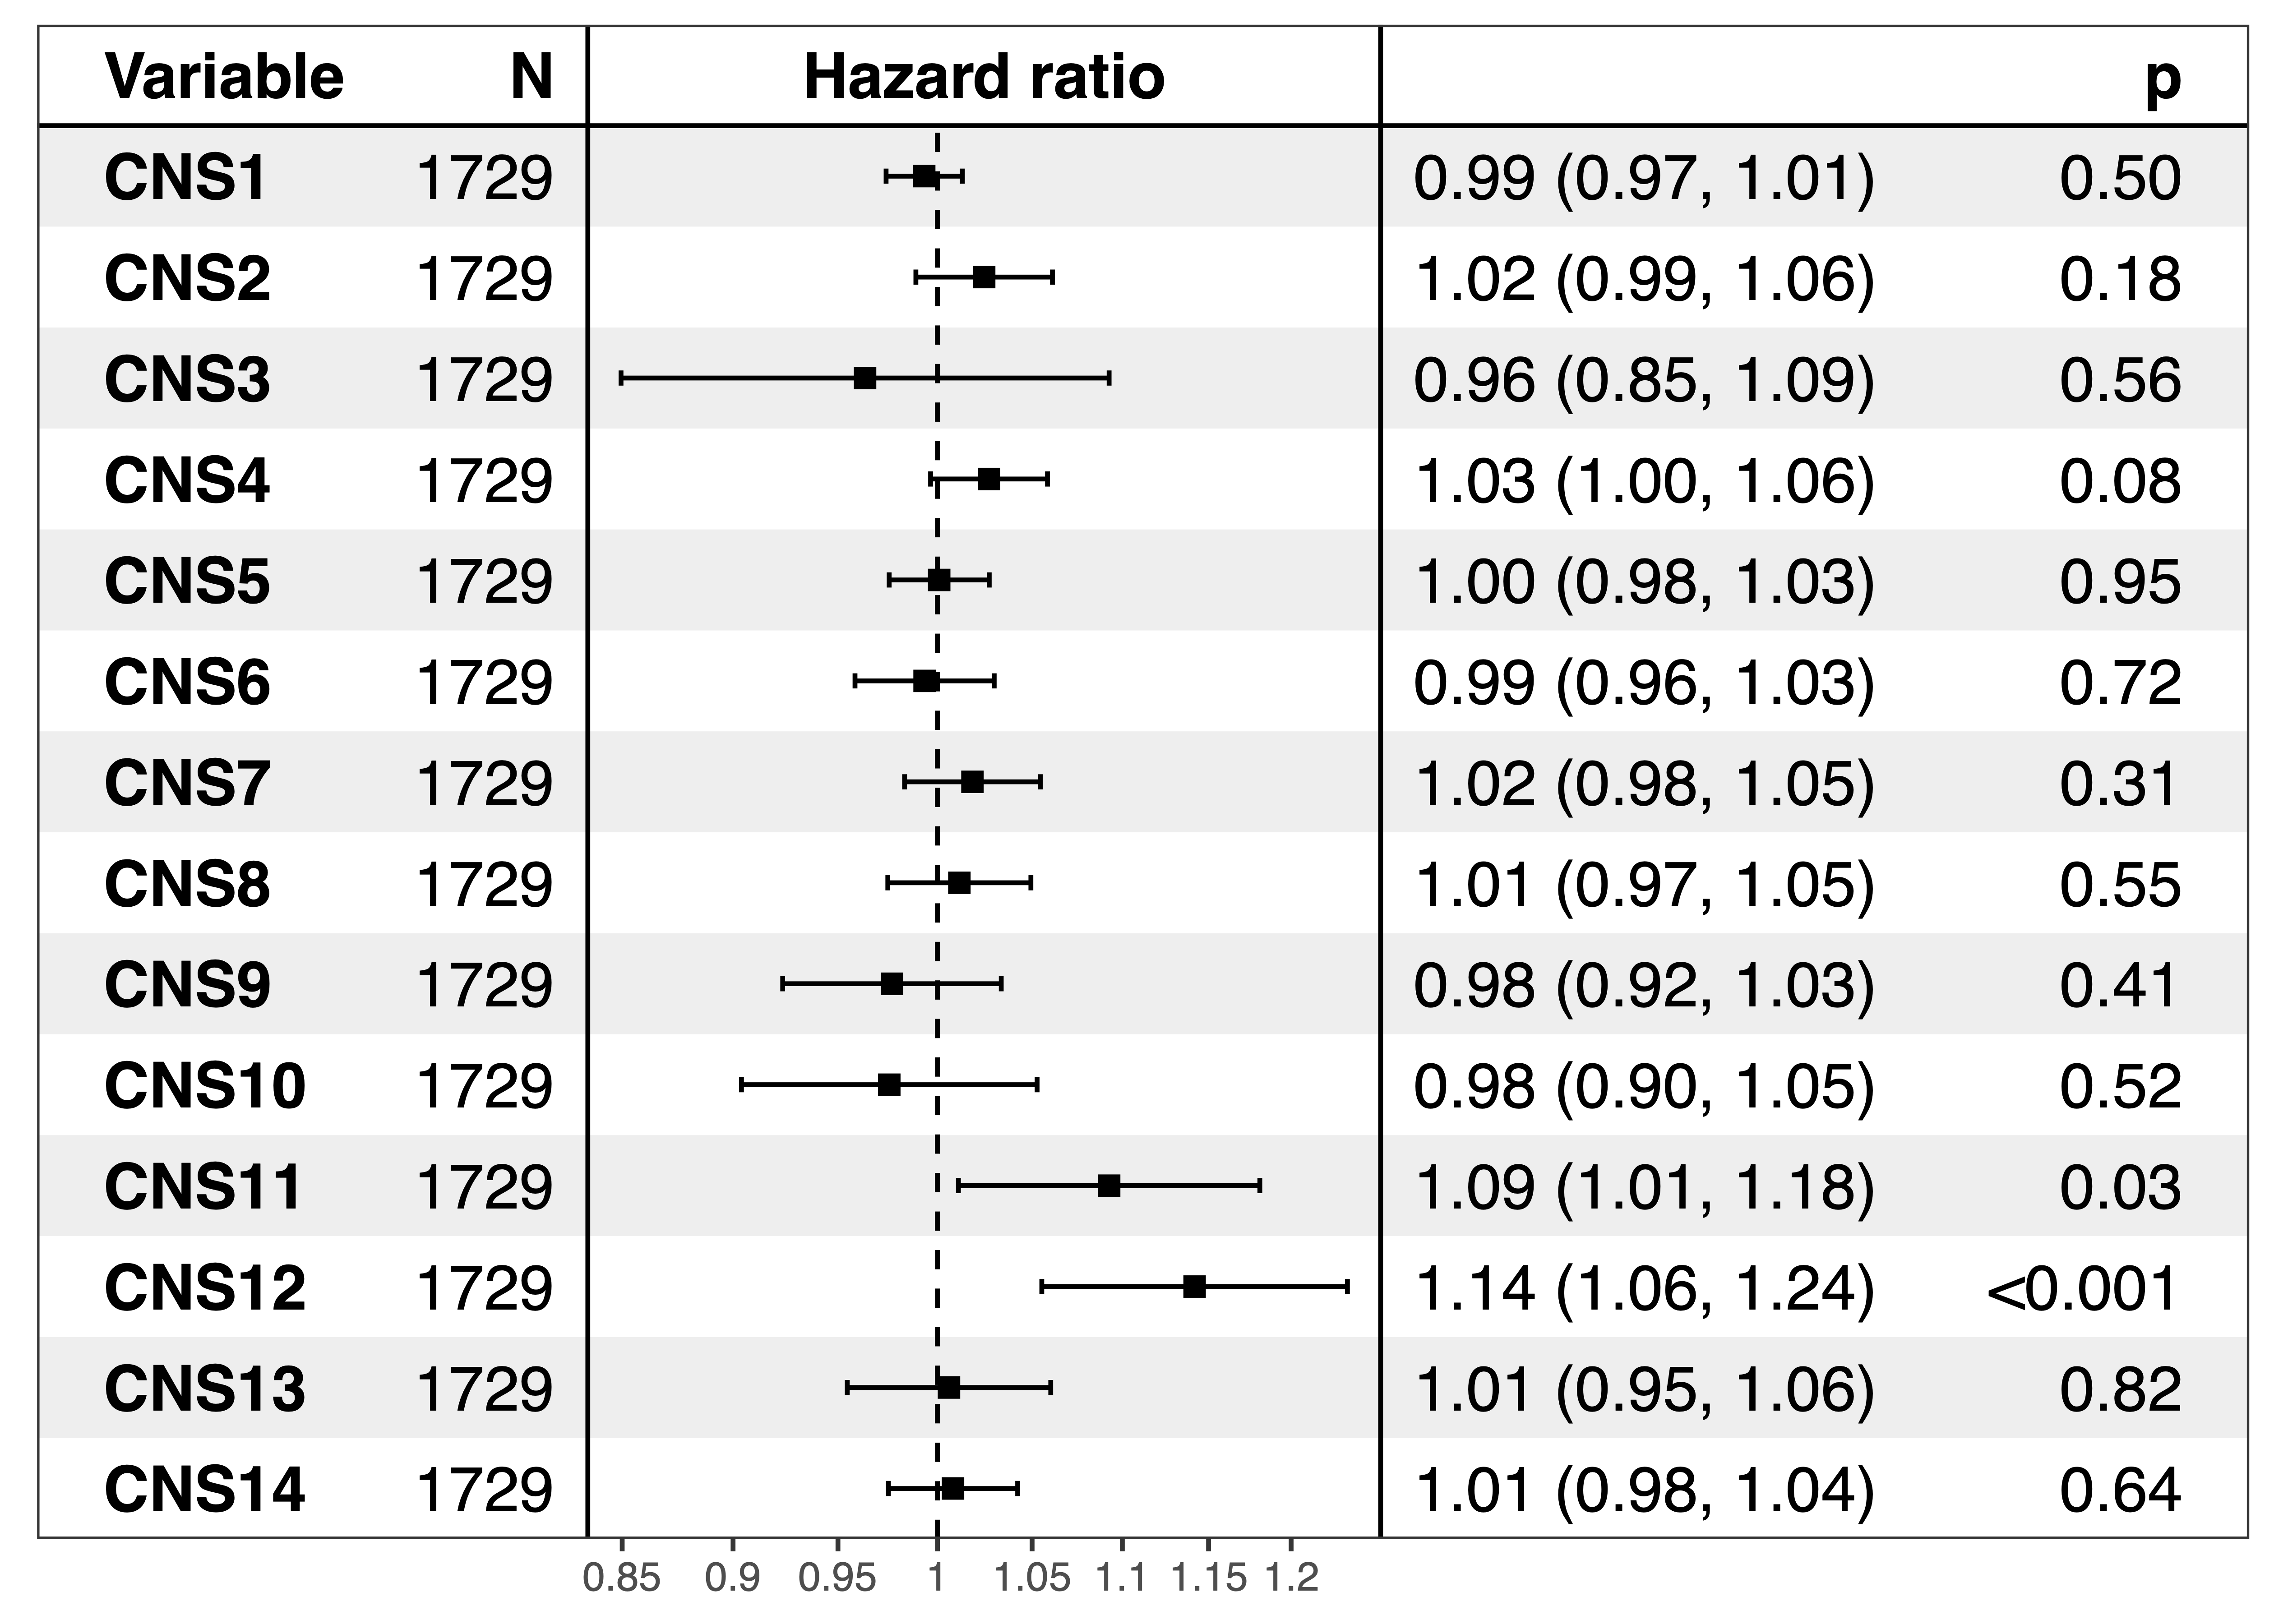
\includegraphics[width=0.8\linewidth]{Figures/pcawg_cox} 

}

\caption{CNA signature activity and cancer patients’ prognosis.}\label{fig:figure5}
\end{figure}

The CNA signatures extracted from cancer patients could be cancer
prognosis biomarkers.In pan-cancer level, activities of CNS11, CNS12 are
significantly associated with poor OS.

\hypertarget{conclusion}{%
\section{Conclusion}\label{conclusion}}

\begin{itemize}
\tightlist
\item
  We developed a unified and comprehensive method for copy number
  signature analysis.
\item
  Our method can be applied in cancer patients with copy number profiles
  generated with WGS, WES or SNP array data. - Our copy number signature
  analysis method is based on a novel and comprehensive method to
  catalog copy number segments.
\item
  copy number signatures could be biomarkers to guide cancer precision
  medicine.
\end{itemize}

\hypertarget{more}{%
\section{More}\label{more}}

You can scan QR code at bottom center to see online analysis report. All
code and related data are published at
\url{https://github.com/XSLiuLab/Pan-cancer_CNA_signature}.

\hypertarget{acknowledgments}{%
\section{Acknowledgments}\label{acknowledgments}}

We thank ShanghaiTech University High Performance Computing Public
Service Platform for computing services. This work was supported by The
National Natural Science Foundation of China (31771373), Shanghai
Science and Technology Commission (21ZR1442400), and startup funding
from ShanghaiTech University.

\hypertarget{recent-works-of-out-lab}{%
\section{Recent works of out lab}\label{recent-works-of-out-lab}}

\begin{itemize}
\tightlist
\item
  Wang, Shixiang, et al.~``Copy number signature analysis tool and its
  application in prostate cancer reveals distinct mutational processes
  and clinical outcomes.'' PLoS genetics 17.5 (2021): e1009557.
\item
  Wang, Shixiang, et al.~``UCSCXenaShiny: an R/CRAN package for
  interactive analysis of UCSC xena data.'' Bioinformatics (2021).
\item
  Wang, Shixiang, et al.~``Sigflow: an automated and comprehensive
  pipeline for cancer genome mutational signature analysis.''
  Bioinformatics 37.11 (2021): 1590-1592.
\end{itemize}

\href{https://github.com/XSLiuLab/}{©Cancer Biology Group} 2021

Research group led by Xue-Song Liu in ShanghaiTech. University. Lab
website is shown in QR code at bottom right.

\end{document}
